% to choose your degree
% please un-comment just one of the following
\documentclass[bsc,logo,frontabs,twoside,singlespacing,normalheadings,parskip]{infthesis}     % for BSc, BEng etc.
% \documentclass[minf,frontabs,twoside,singlespacing,parskip]{infthesis}  % for MInf

% FONT COMMANDS
\usepackage{fontspec}
\setmainfont[Mapping=tex-text,Numbers=OldStyle]{fbb}
\setsansfont[Mapping=tex-text,Numbers=OldStyle,Scale=MatchLowercase]{Gill Sans}
\setmonofont[Mapping=tex-text,Scale=MatchLowercase]{Inconsolata}

\usepackage{epsfig}

% ENSURE CHAPTERS WORK IN PDF VIEWERS
\usepackage[]{hyperref}
\hypersetup{
    pdftitle={Storm on Multi-core},
    pdfauthor={Mark Nemec},
    %pdfsubject={Your subject here},
    %pdfkeywords={keyword1, keyword2},
    bookmarksnumbered=true,
    bookmarksopen=true,
    bookmarksopenlevel=1,
    %colorlinks=true,
    pdfstartview=Fit,
    pdfpagemode=UseOutlines,
    pdfpagelayout=TwoPageRight
}

\begin{document}

\title{Storm on Multi-core}

\author{Mark Nemec}

% to choose your course
% please un-comment just one of the following
% \course{Artificial Intelligence and Computer Science}
%\course{Artificial Intelligence and Software Engineering}
%\course{Artificial Intelligence and Mathematics}
%\course{Artificial Intelligence and Psychology }
%\course{Artificial Intelligence with Psychology }
%\course{Linguistics and Artificial Intelligence}
\course{Computer Science}
%\course{Software Engineering}
%\course{Computer Science and Electronics}
%\course{Electronics and Software Engineering}
%\course{Computer Science and Management Science}
%\course{Computer Science and Mathematics}
%\course{Computer Science and Physics}
%\course{Computer Science and Statistics}

% to choose your report type
% please un-comment just one of the following
%\project{Undergraduate Dissertation} % CS&E, E&SE, AI&L
%\project{Undergraduate Thesis} % AI%Psy
\project{4th Year Project Report}

\date{\today}

\abstract{
This is an example of {\tt infthesis} style.
The file {\tt skeleton.tex} generates this document and can be
used to get a ``skeleton'' for your thesis.
The abstract should summarise your report and fit in the space on the
first page.
%
You may, of course, use any other software to write your report,
as long as you follow the same style. That means: producing a title
page as given here, and including a table of contents and bibliography.
}

\maketitle

\section*{Acknowledgements}
Acknowledgements go here.

\tableofcontents

\pagenumbering{arabic}


%%%%%%%%%%%%%%%%%%%%%%%%%%%%%%%%%%%%%%%%%%%%%
%%
%%				INTRODUCTION
%%
%%%%%%%%%%%%%%%%%%%%%%%%%%%%%%%%%%%%%%%%%%%%%


\chapter{Introduction}

In recent years, there has been an explosion of cloud computing software. After Google published their paper on MapReduce \cite{Anonymous:Jj3E6x7v}, many new open-source frameworks for distributed computation have emerged, most notably Apache Hadoop for batch processing and Apache Storm for real-time data stream processing.

The main idea of these frameworks is to split the work that needs to be carried out and distribute it across multiple nodes of a cluster. Commercial companies and researchers have been able to utilise these frameworks and create distributed systems \cite{5billion-sessions} which can accomplish things that would not be possible on a single computer. This has mostly been allowed by the low price of commodity hardware and good horizontal scaling properties.

% TODO: Here talk about What this paper is about !
% TODO: Maybe mention the Hadoop multi-core paper
% TODO: Maybe a section - move main idea here?
This project is about taking the ideas from the distributed system Apache Storm and applying them in the context of multi-core machines instead of clusters.

%% TODO: After that comes Motivation which explains why it's a good idea!
\section{Motivation}

While the cost of a commodity hardware cluster might be lower than the price of a single computer with equal power there are certain limitations:

\begin{itemize}

\item The nodes of a cluster communicate through network. This limits the speed of communication between processes that live on different nodes.

\item Distributed systems waste resources by replicating data to ensure reliability.

% TODO: Maybe mention renting vs owning here
\item Running a distributed computation on commodity hardware usually requires a data centre or renting out instances on cloud computing services such as Amazon EC2 or Rackspace. This is not ideal for some use cases which require full control over the system or a heightened level of security. 

\end{itemize}

On the other hand, even though Moore’s law still holds true, processor makers now favour increasing the number of cores in CPU chips to increasing their frequency. This trend implies that the “free lunch” of getting better software performance by upgrading the processor is over and programmers now have to design systems with parallel architectures in mind. However, there are some limitations to this as well:

\begin{itemize}

\item It is generally believed that writing parallel software is hard. The traditional techniques of message passing and parallel threads sharing memory require the programmer to manage the concurrency at a fairly low level, either by using messages or locks.

%% TODO: Rephrase "nice if they could"
\item Apache Storm has become the de facto tool used in stream processing on a cluster and according to their "Powered By" page \cite{Anonymous:eikzOt4-} there are tens of companies already using Storm to process their real-time streams. It would be nice if they could keep that code.

\end{itemize}

\section{Main Idea}

The solution proposed in this paper is to take the existing Apache Storm project and port it for multi-core machines. This is implemented in a library Storm-MC with an API compatible with Apache Storm. This allows us to take an existing application written with Apache Storm in mind and run it in a multi-core setting. This way, we can avoid network latency and enjoy the significant performance improvements of a shared-memory environment.

\begin{itemize}

	\item Prices of high-end server have decreased and one can get a 32-core machine for 10,000 USD.

\end{itemize}

\section{Structure of the Report}
%% And after that explain the structure of the report :)

In chapter 1, blah blah.


%%%%%%%%%%%%%%%%%%%%%%%%%%%%%%%%%%%%%%%%%%%%%
%%
%%				BACKGROUND
%%
%%%%%%%%%%%%%%%%%%%%%%%%%%%%%%%%%%%%%%%%%%%%%


\chapter{Background}

In this chapter we give background information necessary to understand the design of Storm-MC.

\section{Core Concepts}

There are several core concepts used by Storm and hence by extension Storm-MC as well. The concepts are put together to form a simple API that allows the user to break down a computation into separate components and then define how these components interact with each other.

\begin{description}
  \item[Spout] A spout is a component that represents the source of a data-stream. Typically, a spout reads from a message broker such as RabbitMQ or Kafka but can also generate its own stream or read from somewhere like the Twitter streaming API.
  \item[Bolt] A bolt is a component that takes a data-stream as an input and transforms it into a different stream for its output. A bolt can perform a range of functions e.g. filter out tuples based on some criteria or perform a join of two different input streams.
  \item[Topology] The programmer connects these components in a directed acyclic graph called topology which describes how the components interact with each other. The topology is then submitted to Storm.
\end{description}

\begin{figure}[!htb]
	\centering
	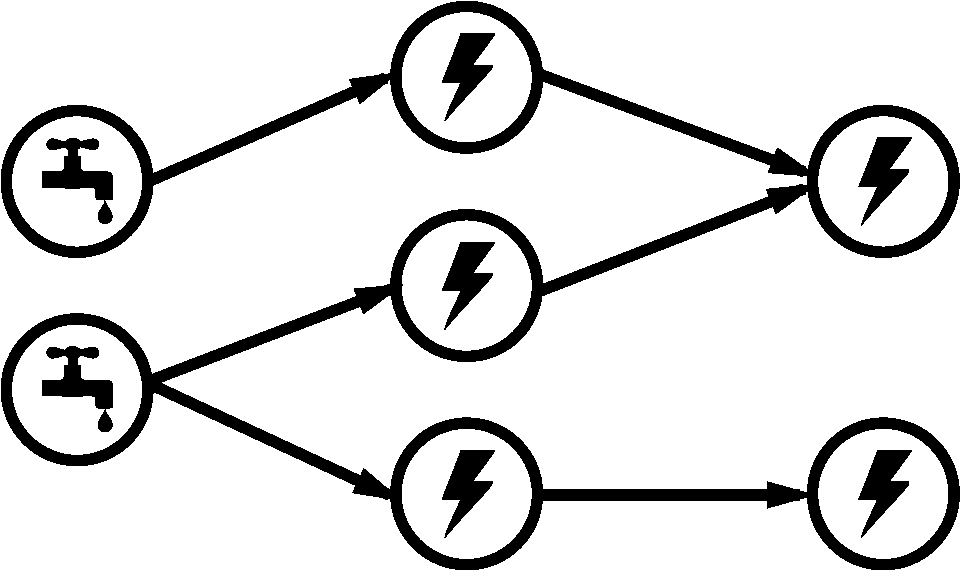
\includegraphics[scale=0.3]{pdf/topology.pdf}
	\caption{An example topology.}
	\label{fig:topology}
\end{figure}

\section{Additional Concepts}

\begin{description}
  \item[Stream] A stream is defined as an unbounded sequence of tuples. Streams can be thought of as edges connecting the bolts and spouts which act as vertices.
  \item[Tuple] A tuple wraps named fields and their values. The values of fields can be of different types. When a component emits a tuple to a stream it sends that tuple to every bolt subscribed to the stream.
  \item[Stream Grouping] Every bolt needs to have a type of stream grouping associated with it. This grouping decides the means of distributing the tuples coming from its input streams amongst the instances of the bolt task.
  	  %% TODO: Maybe list Grouping types
\end{description}

All the components of a Storm topology execute in parallel. A user can specify how much parallelism he wants associated with every component and Storm spawns the necessary number of threads.

\section{Storm Architecture}

%% TODO: Maybe highlight similarities to Hadoop

The Storm cluster uses a Master-Worker pattern. The master node runs a daemon called Nimbus which receives topologies submitted by clients, makes task assignments to worker nodes, and monitors them for failure. The worker nodes run a daemon called Supervisor which spawns worker processes which execute the tasks assigned to them. Lastly, the cluster contains a number of Zookeeper nodes which coordinate the communication between the master and the workers.

\subsection{Nimbus Node}

The master node (also called Nimbus) is responsible for the following tasks:

\begin{enumerate}
	\item Receive a submission with a topology and configuration from programmer.
	\item Distribute the work performed by different components to worker nodes.
\end{enumerate}

The Nimbus node is fault tolerant
%% TODO: Describe what Nimbus node does.

\subsection{Worker Nodes}

The innards of a Worker node are as follows:

\begin{description}
	\item[Supervisor] \hfill \\
	A supervisor is a daemon process, run under supervision, that launches worker processes. This daemon is what the user runs on a worker node to make it part of the cluster.
	\item[Worker] \hfill \\
	A worker is a process that is assigned a port and listens to tuple messages on a socket associated with the port. Whenever it receives a tuple, it puts it on a queue where it is picked up by one or more executors of the worker process.
	\item[Executor] \hfill \\
	An executor controls the parallelism within a worker process. Every executor runs in a separate thread. Its job is to pick up tuples from the receiving queue, perform the function of a component they represent, and put the transformed tuples on the transfer queue, ready to be sent along to the next component. An executor runs one (the usual case) or more tasks.
	\item[Task] \hfill \\
	A task performs the actual data processing. However, within an executor thread all the tasks are executed sequentially. The main reason for having tasks is that the number of tasks stays the same throughout the lifetime of a topology but the number of executors can change (by rebalancing). Thus if some worker nodes in the cluster go down, the topology can continue executing with the same number of tasks as before.
\end{description}

\subsection{Zookeeper Nodes}

%% TODO: Describe how zookeeper nodes work.
The Zookeeper nodes can be thought of as the glue of the network. They ensure that messages are delivered.

\section{Serialisation}

Since Storm topologies execute on a cluster all the components need to be serialisable. This is achieved with Apache Thrift. Thus, components are defined as Thrift objects and Thrift generates all the Java serialisation code automatically.


%%%%%%%%%%%%%%%%%%%%%%%%%%%%%%%%%%%%%%%%%%%%%
%%
%%				   DESIGN
%%
%%%%%%%%%%%%%%%%%%%%%%%%%%%%%%%%%%%%%%%%%%%%%


\chapter{Design}

The design of Storm-MC was ported over from Apache Storm. Clearly, however, some differences had to be made to take advantage of a multi-core machine performance. This chapter explains the design of Storm-MC.

\section{Apache Storm on Multi-core}

To begin, we discuss why Apache Storm does not perform well on a single machine. When running on multi-core architectures, Storm runs in local mode. There are several reasons why the local mode is not as performant as it could be.

\begin{description}
	\item[Multi-process Nature of Storm] \hfill \\
	In general, multi-process applications suffer overhead from inter-process communication and are generally slower than their multi-threaded counterparts\cite{gluck_optimization_????}.
	%% TODO: This could be another disadvantage
%	\item[Serialisable components] \hfill \\
	\item[Redundant threads] \hfill \\
	Storm runs many threads which are only useful in distributed context. Indeed, during our experiments we found that a topology with 8 executors was being executed with 64 threads. This included threads which were used as timeout timers or to send heartbeats and were unnecessary in a multi-core setting. Obviously, not all of them were executing in parallel but there is clearly room for reduction.
	%% TODO: Probably a link here
	%% TODO: Maybe include Thread Dump
	%% TODO: Also mention Acker not even running
	%% TODO: Maybe mention how many threads with Storm-MC
\end{description}

\section{Storm-MC Architecture}

The overall architecture of Storm-MC can be seen in figure.

\begin{figure}[!htb]
	\centering
	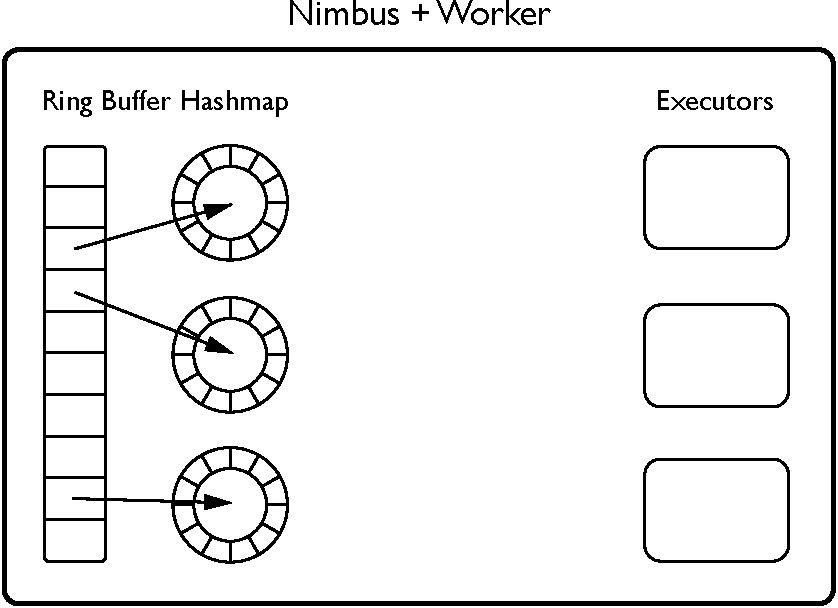
\includegraphics[scale=0.7]{pdf/storm_mc_arch.pdf}
	\caption{Storm-MC Architecture.}
	\label{fig:architecture}
\end{figure}

\subsection{Main Process}

%%%%%%%%%%%%%%%%%%%%%%%%%%%%%%%%%%%%%%%%%%%%%
%%
%%			    IMPLEMENTATION
%%
%%%%%%%%%%%%%%%%%%%%%%%%%%%%%%%%%%%%%%%%%%%%%


\chapter{Implementation}


%%%%%%%%%%%%%%%%%%%%%%%%%%%%%%%%%%%%%%%%%%%%%
%%
%%				   EVALUATION
%%
%%%%%%%%%%%%%%%%%%%%%%%%%%%%%%%%%%%%%%%%%%%%%


\chapter{Evaluation}


%%%%%%%%%%%%%%%%%%%%%%%%%%%%%%%%%%%%%%%%%%%%%
%%
%%				CONCLUSION
%%
%%%%%%%%%%%%%%%%%%%%%%%%%%%%%%%%%%%%%%%%%%%%%


\chapter{Conclusion}

Of course
you may want to use several chapters and much more text than here.

% use the following and \cite{} as above if you use BibTeX
% otherwise generate bibtem entries
\bibliographystyle{plain}
\bibliography{mybibfile}

\end{document}
